\documentclass[11pt,a4paper]{article}
\usepackage[T1]{fontenc}
\usepackage[portuguese]{babel}
\usepackage[utf8]{inputenc}
\inputencoding{utf8}
\usepackage{url}
%\usepackage{siunitx} % Provides the \SI{}{} and \si{} command for typesetting SI units
\usepackage{graphicx} % Required for the inclusion of images
\usepackage{caption}
\usepackage{subcaption}
\usepackage{natbib} % Required to change bibliography style to APA
\usepackage{enumerate}
\usepackage{amsmath} % Required for some math elements 
\usepackage{graphicx}
\usepackage{epstopdf} %use postscript
\usepackage{float}
\usepackage{a4wide}
\usepackage{amsmath}
\usepackage{amsfonts}
\usepackage{wrapfig}
\usepackage{tikz}
\usetikzlibrary{shapes,arrows,positioning,calc}
\usepackage{amsthm} % Math packages
%\usepackage[headheight=14pt]{geometry}
\usepackage{sectsty} % Allows customizing section commands
\usepackage{fancyhdr} % Custom headers and footers
%\usepackage[margin=1in]{geometry} % Change margin
\pagestyle{fancyplain} % Makes all pages in the document conform to the custom headers and footers
%\fancyhead{} % No page header - if you want one, create it in the same way as the footers below
\fancyhead[L]{Relatório Preliminar}% Empty left footer
\fancyhead[R]{Inteligência Computacional} % Empty center footer
\fancyfoot[C]{\thepage} 								% Page numbering for right footer
\numberwithin{equation}{section}


\begin{document}


\begin{titlepage}

\vspace*{\fill}
 
\newcommand{\HRule}{\rule{\linewidth}{0.5mm}} 	% Defines a new command for the horizontal lines, change thickness here

\center 												% Center everything on the page
 
%----------------------------------------------------------------------------------------
%   LOGO SECTION
%----------------------------------------------------------------------------------------

\includegraphics[scale=0.3]{./minerva}\\[1cm] % Include a department/university logo - this will require the graphicx package
 
%----------------------------------------------------------------------------------------
%   HEADING SECTIONS
%----------------------------------------------------------------------------------------

\textsc{\LARGE Universidade Federal do Rio de Janeiro}\\[1.5cm] % Name of your university/college
\textsc{\Large Inteligência Computacional}\\[0.5cm] % Major heading such as course name
%\textsc{\large   }\\[0.5cm] % Minor heading such as course title

%----------------------------------------------------------------------------------------
%   TITLE SECTION
%----------------------------------------------------------------------------------------

\HRule 
\\[0.8cm]
{ \huge \bfseries  Relatório Preliminar }\\[0.4cm] % Title of your document
\HRule \\[1.5cm]
 
%----------------------------------------------------------------------------------------
%   AUTHOR SECTION
%----------------------------------------------------------------------------------------

\begin{minipage}{0.4\textwidth}
\begin{flushleft} \large
\emph{Nomes:}\\
Aramys Almeida Matos \\
Luís Gustavo Oliveira Silva 
\end{flushleft}
\end{minipage}
~
\begin{minipage}{0.4\textwidth}
\begin{flushright} \large
\emph{Professor:} \\
Alexandre Evsukoff  % Supervisor's Name
\end{flushright}
\end{minipage}\\[4cm]
%----------------------------------------------------------------------------------------
%   DATE SECTION
%----------------------------------------------------------------------------------------


%----------------------------------------------------------------------------------------

%\vfill % Fill the rest of the page with whitespace
\vspace*{\fill}
\end{titlepage}
\section{Introdução}
Este trabalho será desenvolvido sobre o \textit{dataset Breast Cancer Wisconsin (Diagnostic)}. Este \textit{dataset} possui como variáveis características computadas a partir de imagens digitalizadas de exames de mama por punção aspirativa por agulha fina. Ele descreve características do núcleo das células presentes na imagem. 
\section{Caracterização}

\subsection{Dados}
O dataset possui os seguintes dados.

\begin{itemize}
\item ID do paciente.
\item Diagnóstico (Maligno ou benigno codificados como $-1$ e $1$ respectivamente)
\end{itemize}

Atributos das células:
\begin{enumerate}
\item Raio (média das distâncias do centro para pontos no perímetro)
\item Textura
\item Perímetro
\item Área
\item Suavidade
\item Compacidade
\item Concavidade
\item Pontos côncavos
\item Simetria
\item Dimensão Fractal
\end{enumerate}

Para esses 10 atributos é calculado média, erro padrão e o pior valor, resultando em 30 variáveis de entrada. 

O dataset é bem balanceado, apresentando 357 amostras benignas, 212 amostras malignas.

\subsection{Histogramas}

\begin{itemize}
\item Radius
\begin{figure}[H]
\centering
  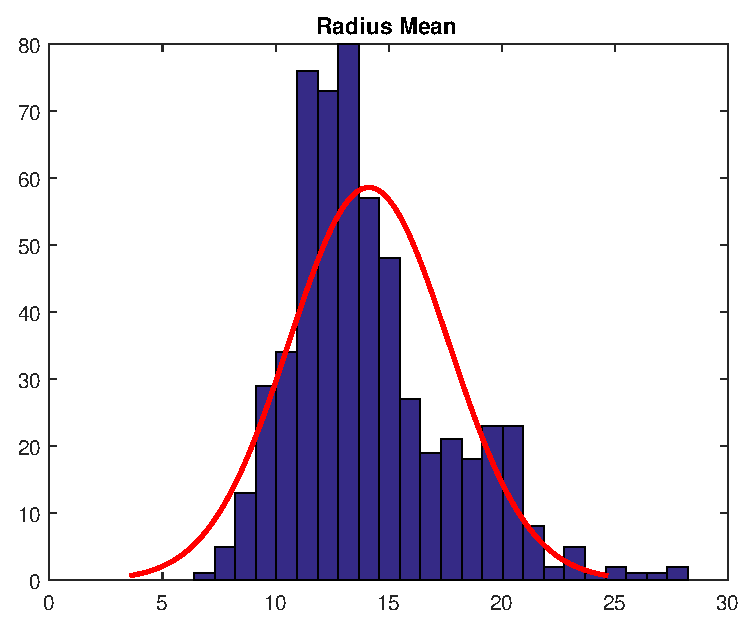
\includegraphics[width=.5\linewidth]{./img/radius_mean}
  \captionof{figure}{Mean}
  \label{fig:test1}
\end{figure}%

\begin{figure}[H]
\centering
\begin{minipage}{.5\textwidth}
  \centering
  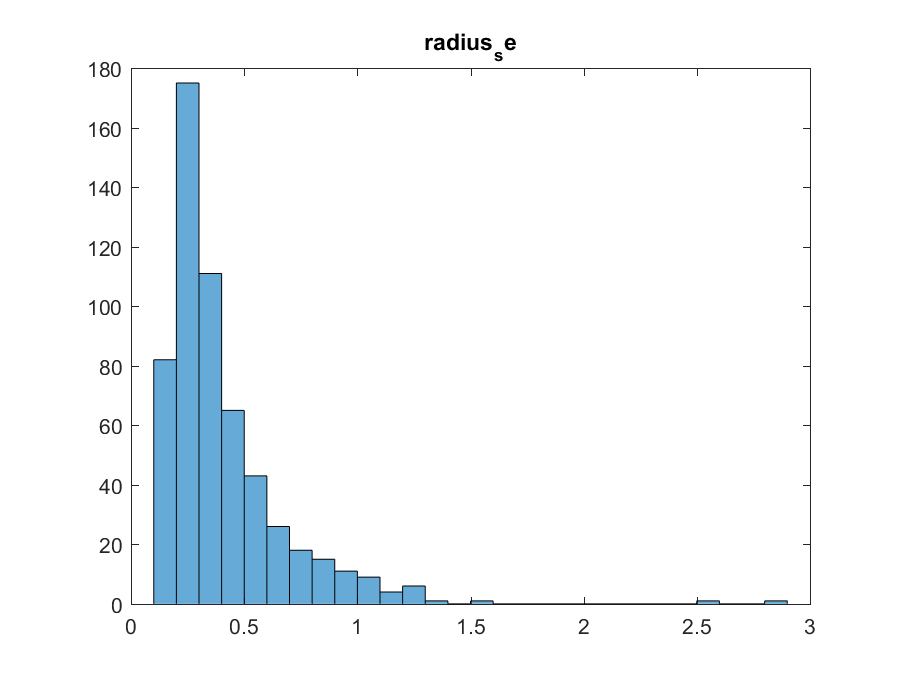
\includegraphics[width=\linewidth]{./img/radius_se}
  \captionof{figure}{Standard Error}
  \label{fig:test1}
\end{minipage}%
\begin{minipage}{.5\textwidth}
  \centering
  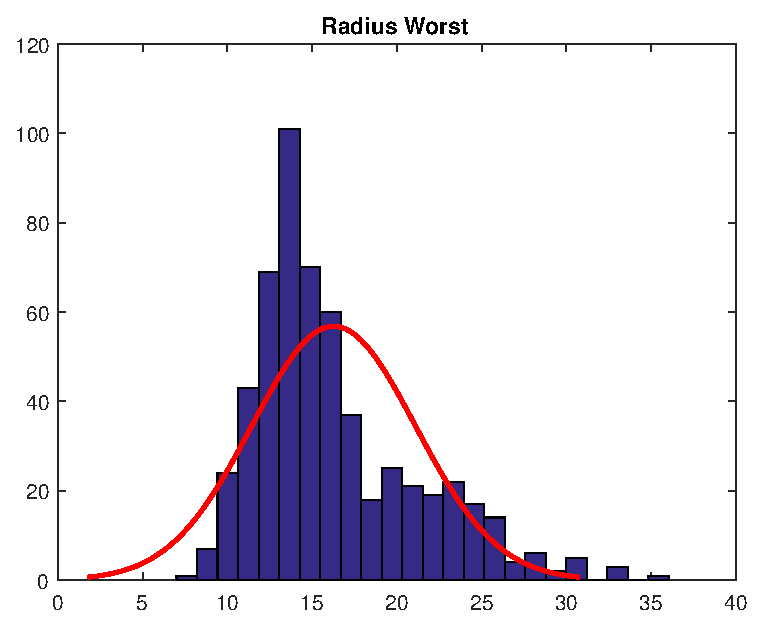
\includegraphics[width=\linewidth]{./img/radius_worst}
  \captionof{figure}{Worst}
  \label{fig:test2}
\end{minipage}
\end{figure}

\item Texture
\begin{figure}[H]
\centering
  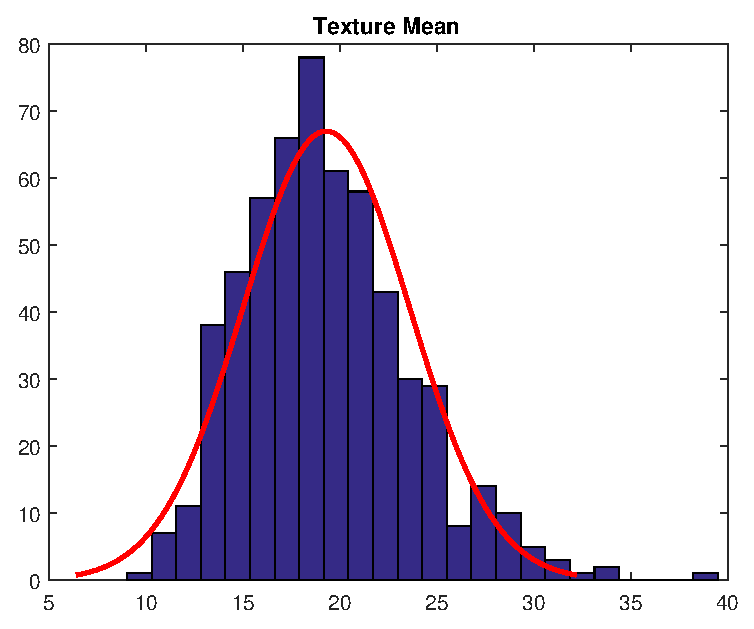
\includegraphics[width=.5\linewidth]{./img/texture_mean}
  \captionof{figure}{Mean}
  \label{fig:test1}
\end{figure}%

\begin{figure}[H]
\centering
\begin{minipage}{.5\textwidth}
  \centering
  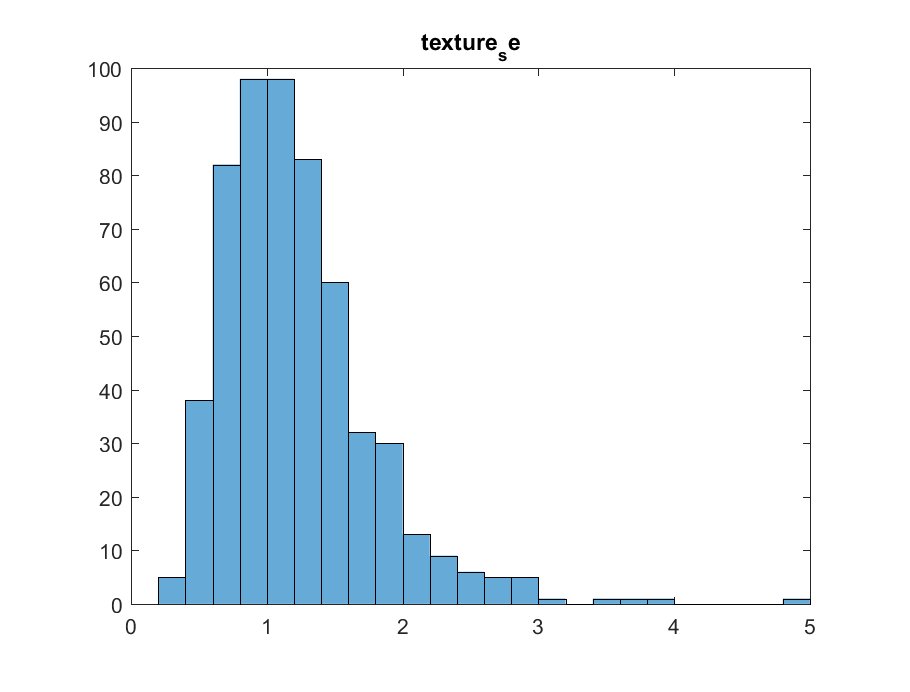
\includegraphics[width=\linewidth]{./img/texture_se}
  \captionof{figure}{Standard Error}
  \label{fig:test1}
\end{minipage}%
\begin{minipage}{.5\textwidth}
  \centering
  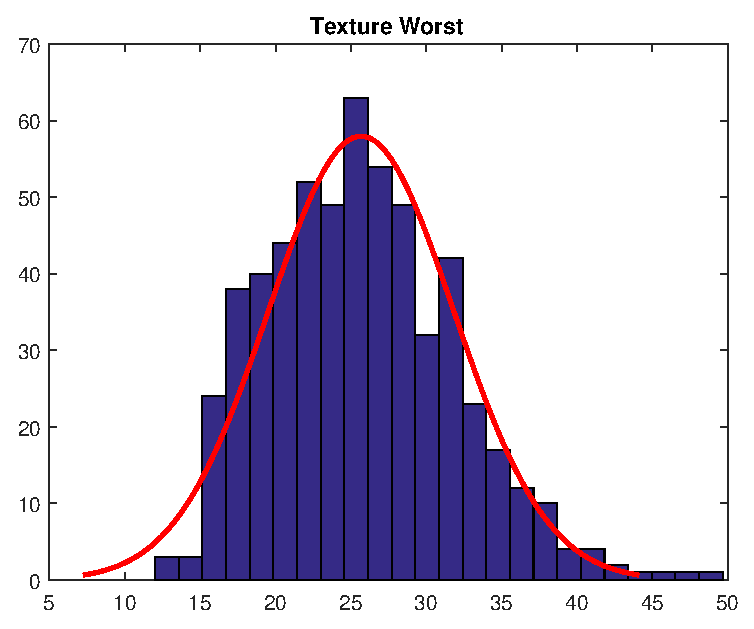
\includegraphics[width=\linewidth]{./img/texture_worst}
  \captionof{figure}{Worst}
  \label{fig:test2}
\end{minipage}
\end{figure}

\item Perimeter
\begin{figure}[H]
\centering
  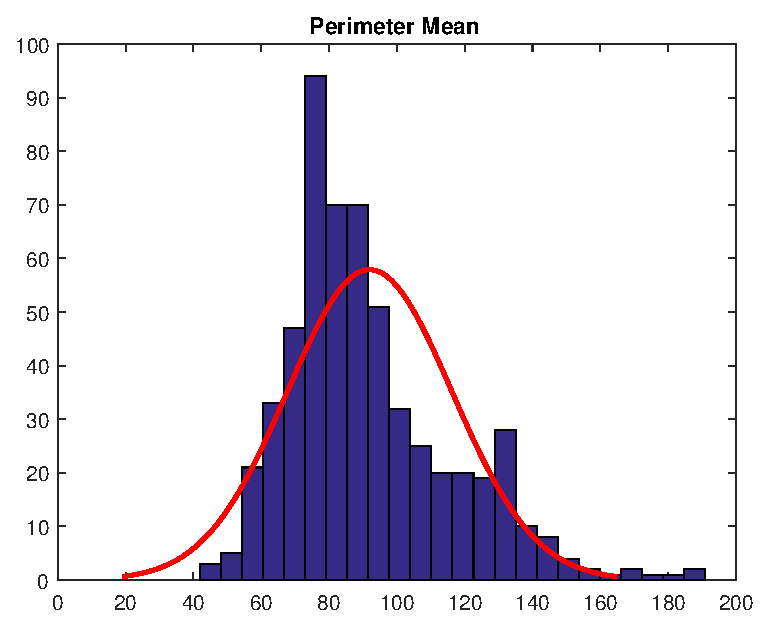
\includegraphics[width=.5\linewidth]{./img/perimeter_mean}
  \captionof{figure}{Mean}
  \label{fig:test1}
\end{figure}%

\begin{figure}[H]
\centering
\begin{minipage}{.5\textwidth}
  \centering
  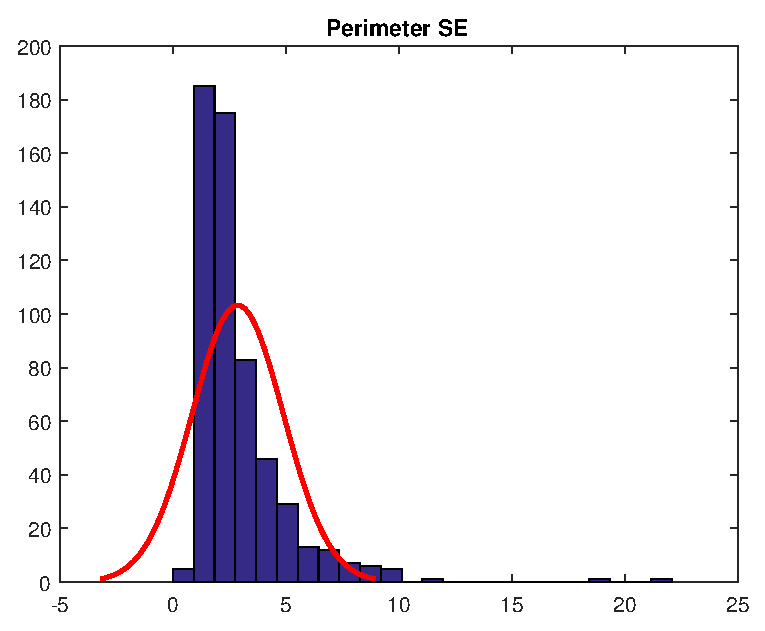
\includegraphics[width=\linewidth]{./img/perimeter_se}
  \captionof{figure}{Standard Error}
  \label{fig:test1}
\end{minipage}%
\begin{minipage}{.5\textwidth}
  \centering
  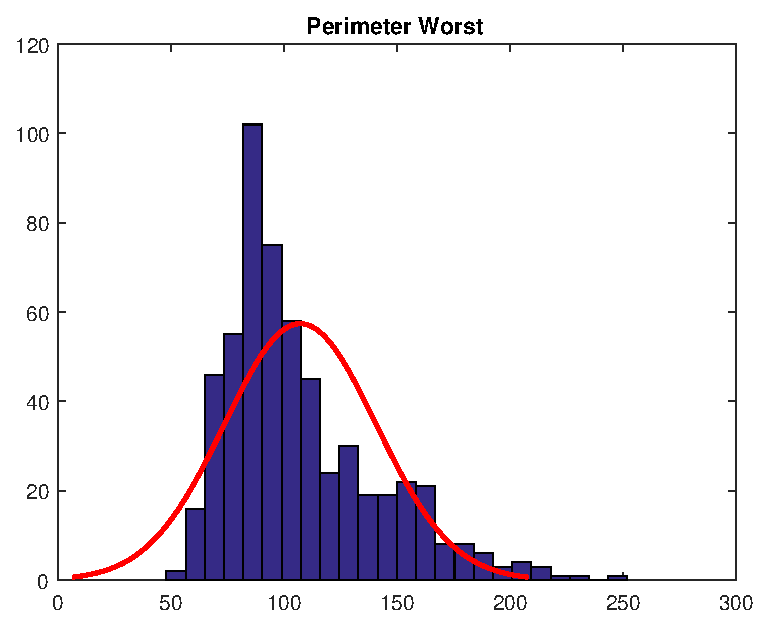
\includegraphics[width=\linewidth]{./img/perimeter_worst}
  \captionof{figure}{Worst}
  \label{fig:test2}
\end{minipage}
\end{figure}

\item Area
\begin{figure}[H]
\centering
  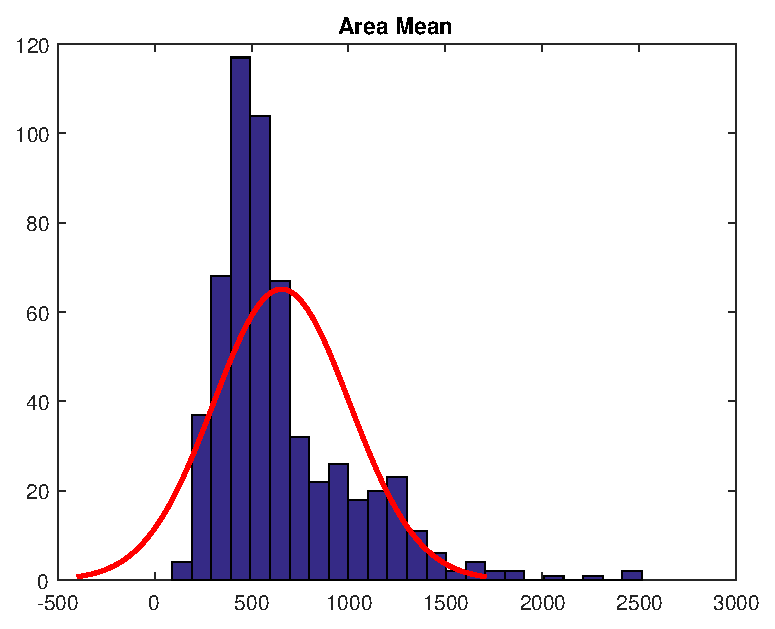
\includegraphics[width=.5\linewidth]{./img/area_mean}
  \captionof{figure}{Mean}
  \label{fig:test1}
\end{figure}%

\begin{figure}[H]
\centering
\begin{minipage}{.5\textwidth}
  \centering
  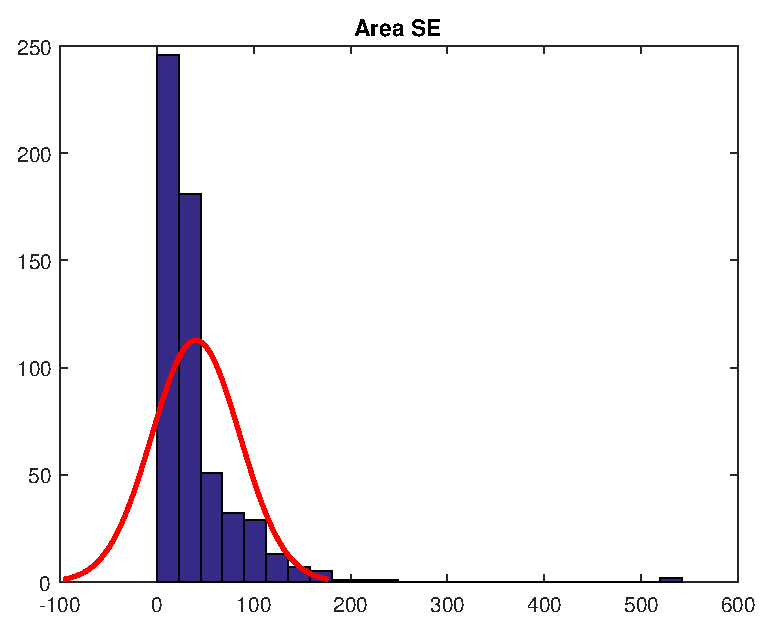
\includegraphics[width=\linewidth]{./img/area_se}
  \captionof{figure}{Standard Error}
  \label{fig:test1}
\end{minipage}%
\begin{minipage}{.5\textwidth}
  \centering
  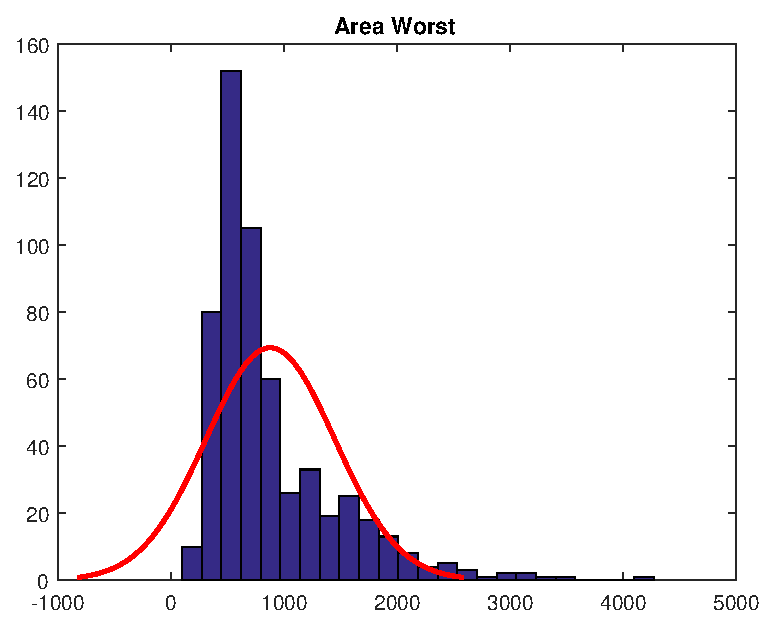
\includegraphics[width=\linewidth]{./img/area_worst}
  \captionof{figure}{Worst}
  \label{fig:test2}
\end{minipage}
\end{figure}

\item Smoothnes
\begin{figure}[H]
\centering
  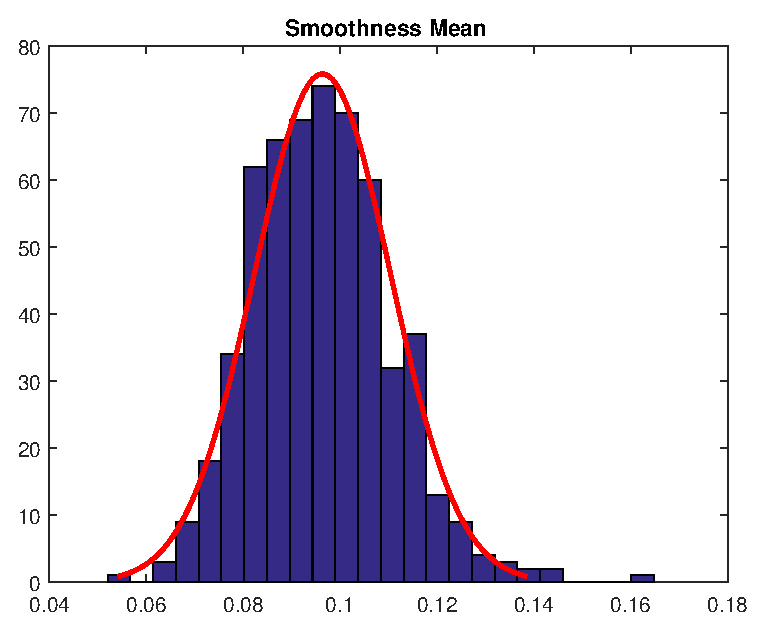
\includegraphics[width=.5\linewidth]{./img/smoothness_mean}
  \captionof{figure}{Mean}
  \label{fig:test1}
\end{figure}%

\begin{figure}[H]
\centering
\begin{minipage}{.5\textwidth}
  \centering
  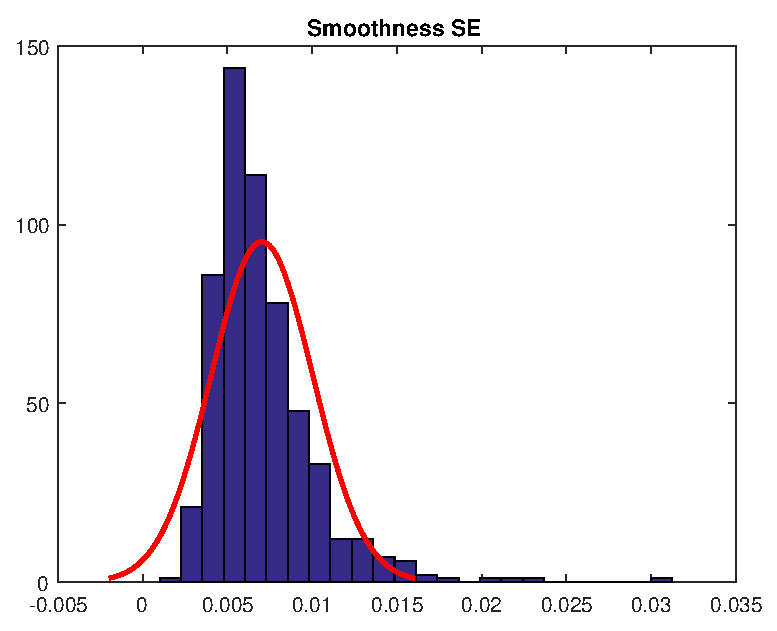
\includegraphics[width=\linewidth]{./img/smoothness_se}
  \captionof{figure}{Standard Error}
  \label{fig:test1}
\end{minipage}%
\begin{minipage}{.5\textwidth}
  \centering
  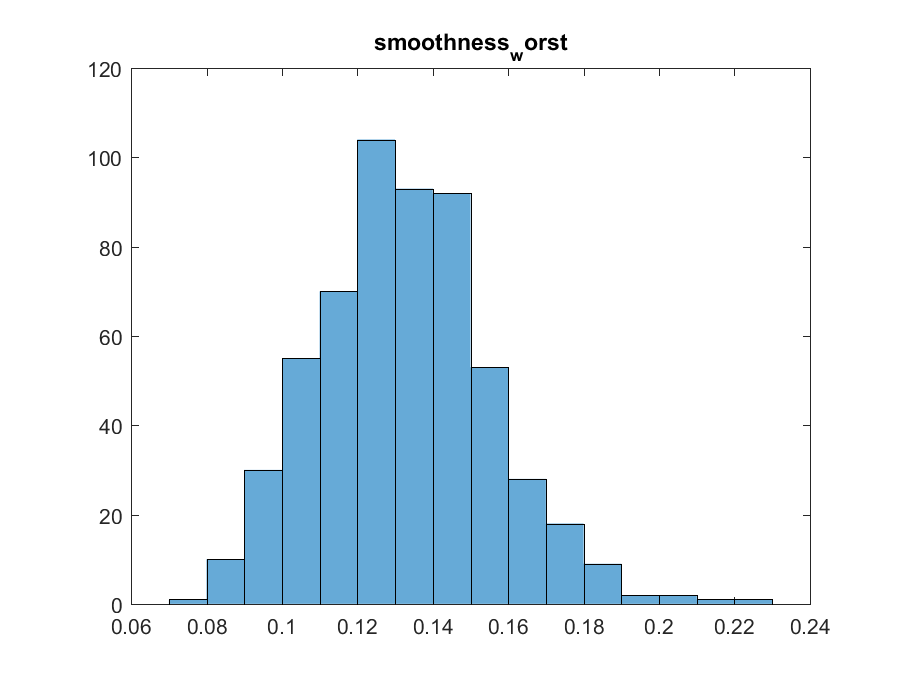
\includegraphics[width=\linewidth]{./img/smoothness_worst}
  \captionof{figure}{Worst}
  \label{fig:test2}
\end{minipage}
\end{figure}

\item Compactness
\begin{figure}[H]
\centering
  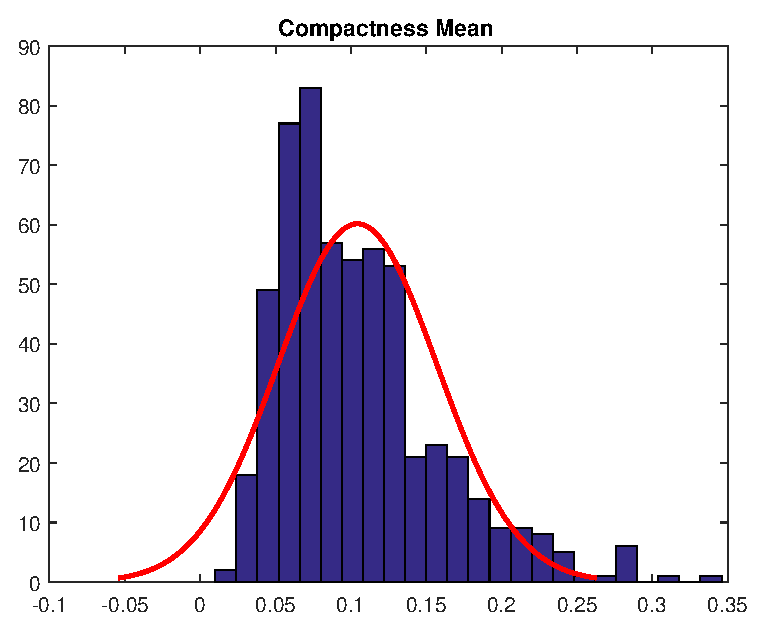
\includegraphics[width=.5\linewidth]{./img/compactness_mean}
  \captionof{figure}{Mean}
  \label{fig:test1}
\end{figure}%

\begin{figure}[H]
\centering
\begin{minipage}{.5\textwidth}
  \centering
  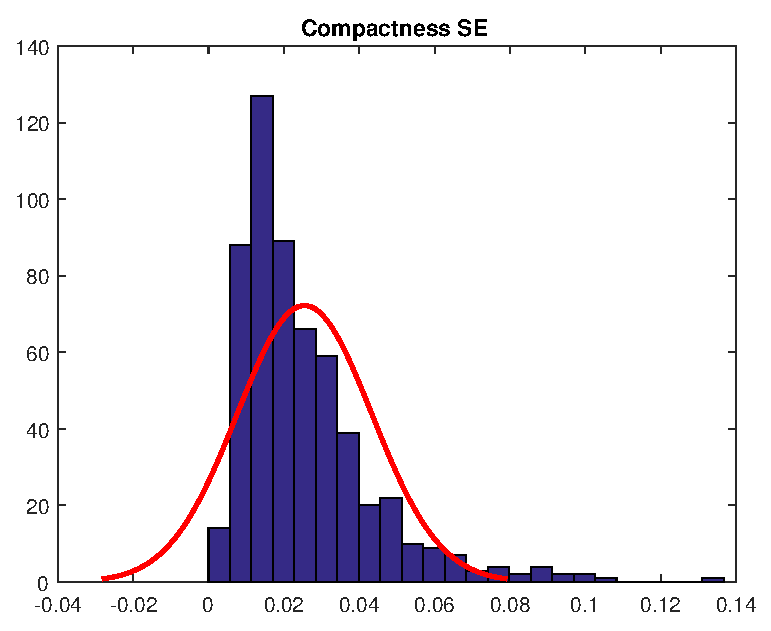
\includegraphics[width=\linewidth]{./img/compactness_se}
  \captionof{figure}{Standard Error}
  \label{fig:test1}
\end{minipage}%
\begin{minipage}{.5\textwidth}
  \centering
  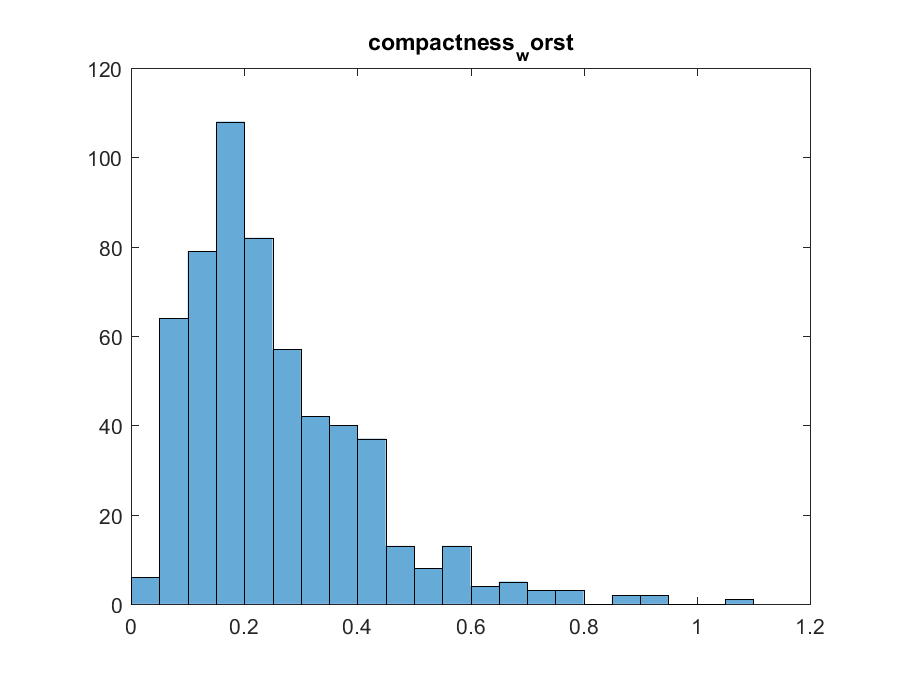
\includegraphics[width=\linewidth]{./img/compactness_worst}
  \captionof{figure}{Worst}
  \label{fig:test2}
\end{minipage}
\end{figure}

\item Concavity
\begin{figure}[H]
\centering
  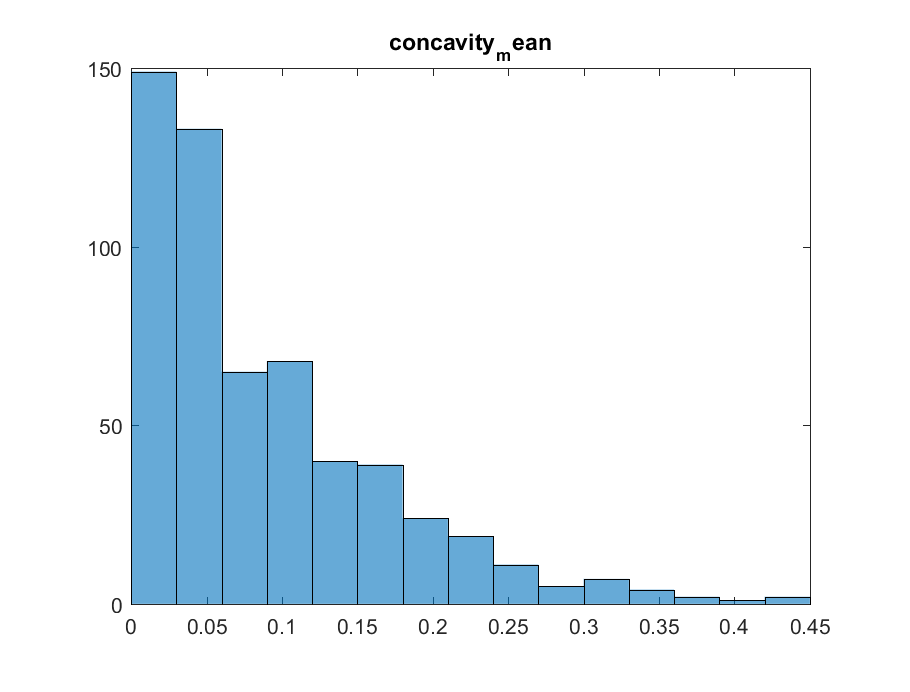
\includegraphics[width=.5\linewidth]{./img/concavity_mean}
  \captionof{figure}{Mean}
  \label{fig:test1}
\end{figure}%

\begin{figure}[H]
\centering
\begin{minipage}{.5\textwidth}
  \centering
  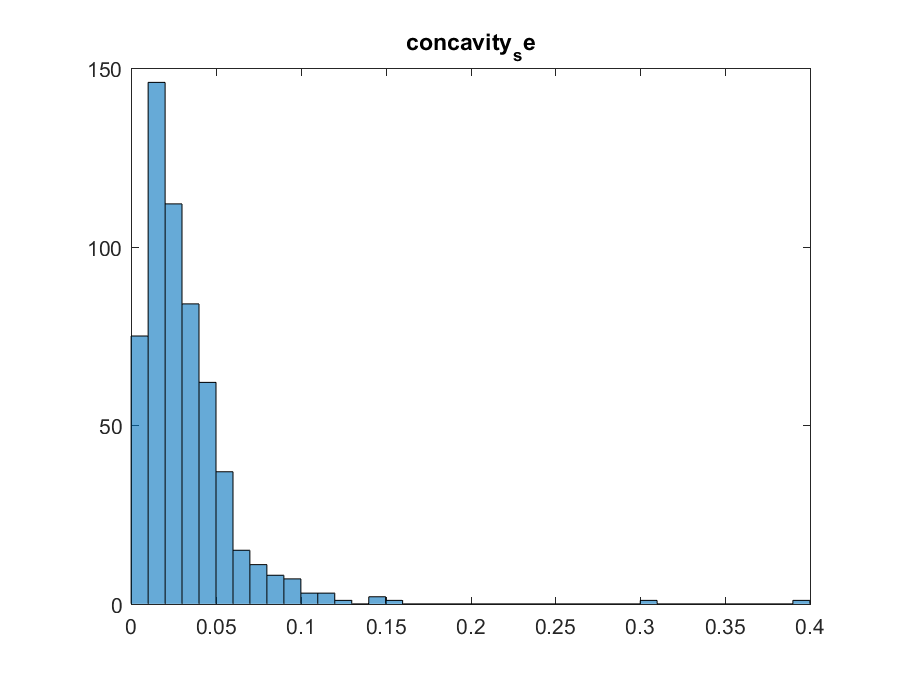
\includegraphics[width=\linewidth]{./img/concavity_se}
  \captionof{figure}{Standard Error}
  \label{fig:test1}
\end{minipage}%
\begin{minipage}{.5\textwidth}
  \centering
  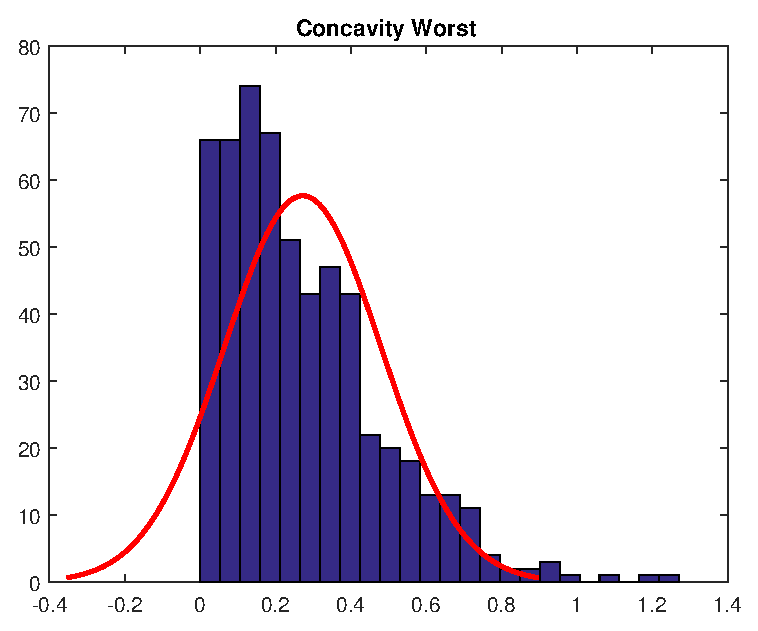
\includegraphics[width=\linewidth]{./img/concavity_worst}
  \captionof{figure}{Worst}
  \label{fig:test2}
\end{minipage}
\end{figure}

\item Concave points
\begin{figure}[H]
\centering
  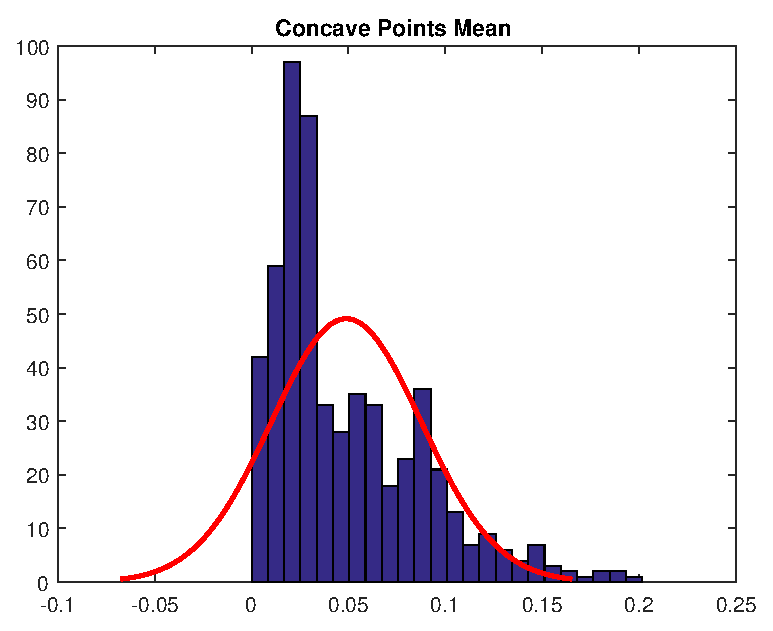
\includegraphics[width=.5\linewidth]{./img/concave_points_mean}
  \captionof{figure}{Mean}
  \label{fig:test1}
\end{figure}%

\begin{figure}[H]
\centering
\begin{minipage}{.5\textwidth}
  \centering
  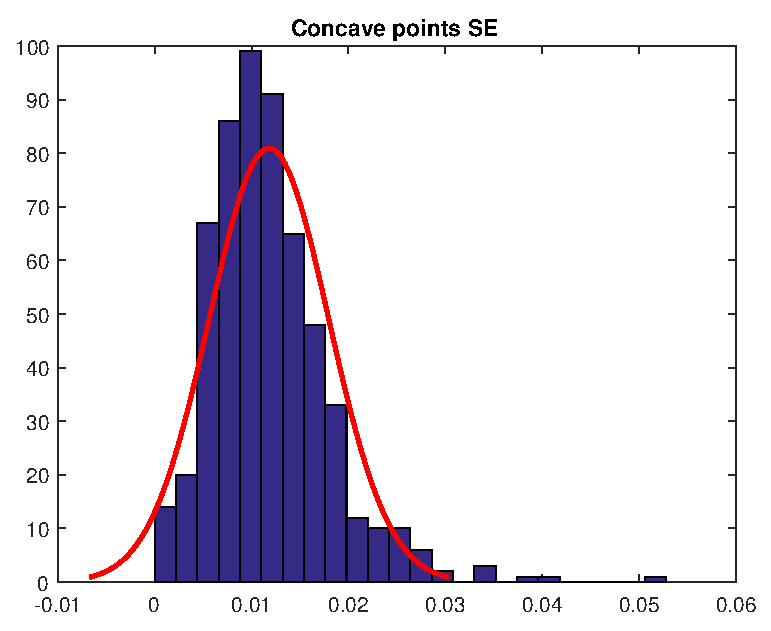
\includegraphics[width=\linewidth]{./img/concave_points_se}
  \captionof{figure}{Standard Error}
  \label{fig:test1}
\end{minipage}%
\begin{minipage}{.5\textwidth}
  \centering
  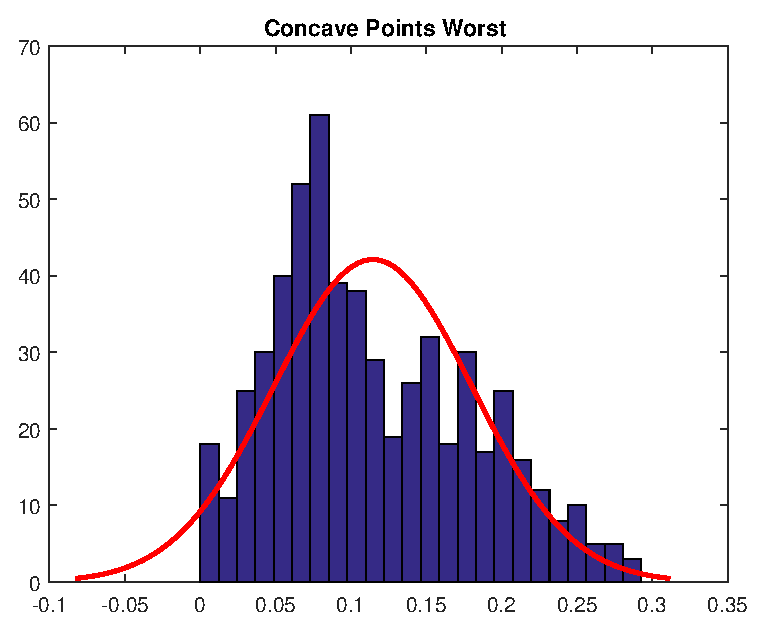
\includegraphics[width=\linewidth]{./img/concave_points_worst}
  \captionof{figure}{Worst}
  \label{fig:test2}
\end{minipage}
\end{figure}


\item Symmetry
\begin{figure}[H]
\centering
  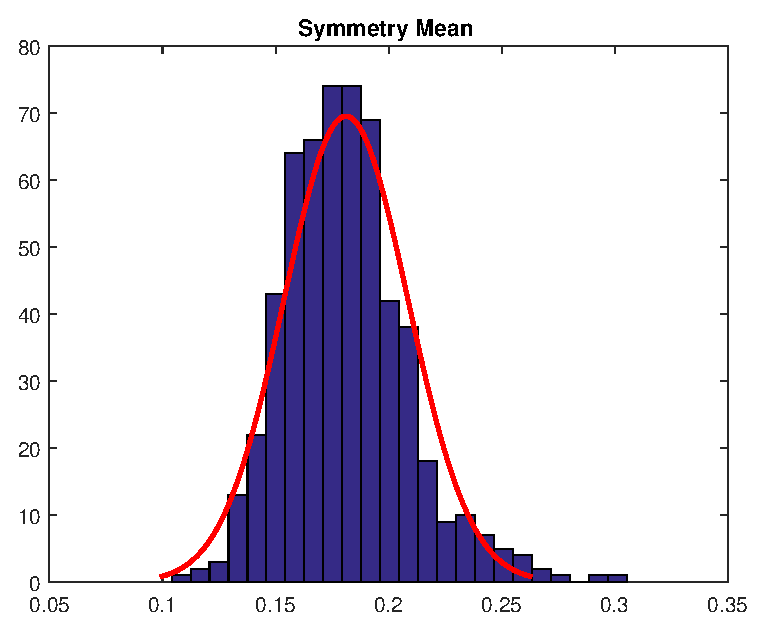
\includegraphics[width=.5\linewidth]{./img/symmetry_mean}
  \captionof{figure}{Mean}
  \label{fig:test1}
\end{figure}%

\begin{figure}[H]
\centering
\begin{minipage}{.5\textwidth}
  \centering
  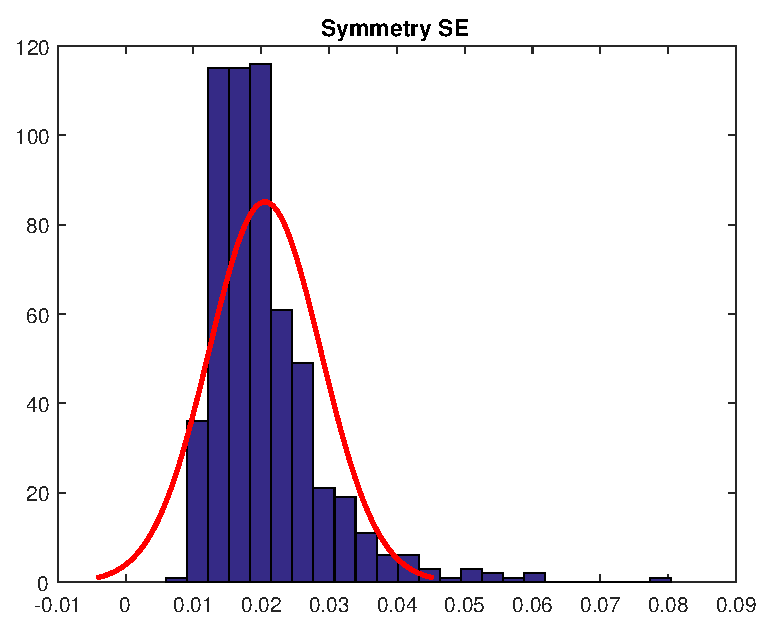
\includegraphics[width=\linewidth]{./img/symmetry_se}
  \captionof{figure}{Standard Error}
  \label{fig:test1}
\end{minipage}%
\begin{minipage}{.5\textwidth}
  \centering
  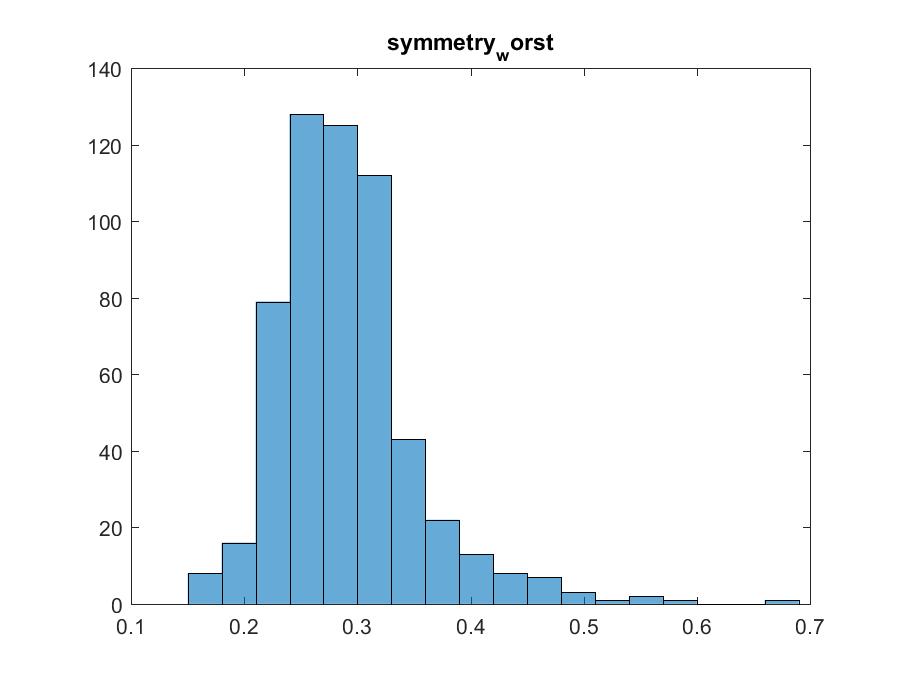
\includegraphics[width=\linewidth]{./img/symmetry_worst}
  \captionof{figure}{Worst}
  \label{fig:test2}
\end{minipage}
\end{figure}

\item Fractal Dimension
\begin{figure}[H]
\centering
  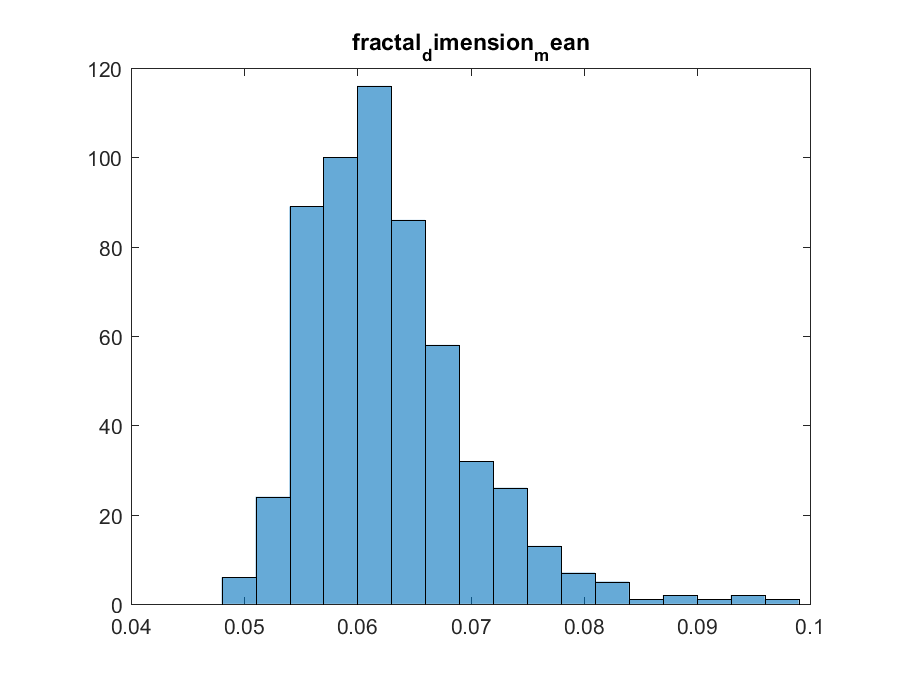
\includegraphics[width=.5\linewidth]{./img/fractal_dimension_mean}
  \captionof{figure}{Mean}
  \label{fig:test1}
\end{figure}%

\begin{figure}[H]
\centering
\begin{minipage}{.5\textwidth}
  \centering
  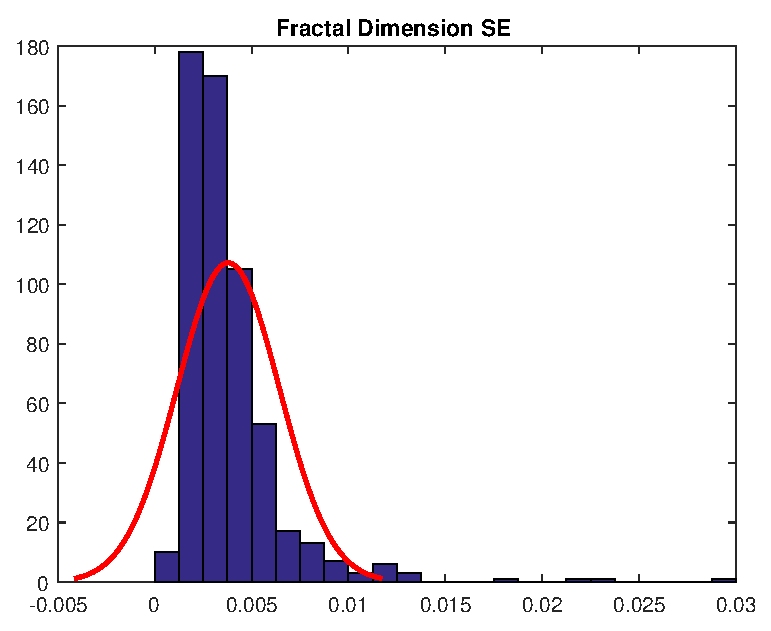
\includegraphics[width=\linewidth]{./img/fractal_dimension_se}
  \captionof{figure}{Standard Error}
  \label{fig:test1}
\end{minipage}%
\begin{minipage}{.5\textwidth}
  \centering
  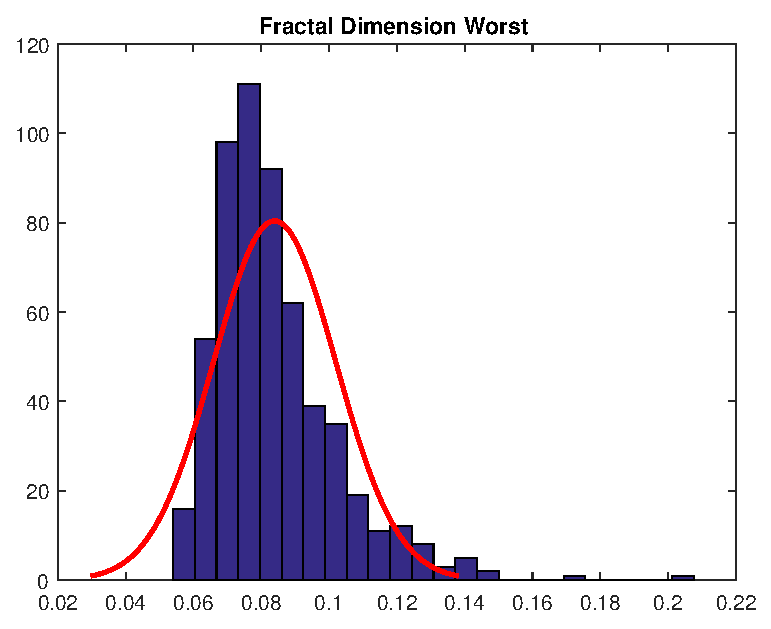
\includegraphics[width=\linewidth]{./img/fractal_dimension_worst}
  \captionof{figure}{Worst}
  \label{fig:test2}
\end{minipage}
\end{figure}
\end{itemize}

\subsection{Matriz de Correlação}
\begin{figure}[H]
\centering
  \includegraphics[width=\linewidth]{./img/corrcoef.png}
  \captionof{figure}{Matriz de Correlação}
  \label{fig:test1}
\end{figure}%

\section{Formulação do Problema}
Consiste em um problema de classificação. Deseja-se desenvolver um classificador capaz de predizer a classe do registro (maligno ou benigno).

Para solução deste problema serão aplicados os modelos de classificação a seguir e avaliados os resultados.
\subsection{Classificador Bayesiano Simples}
\subsection{Classificador Bayesiano Quadrático}
\subsection{Mínimos Quadrados}
\subsection{Regressão Logística}

\section{Apresentação da Tecnologia}
Para a implementação e execução dos algoritmos serão usadas as seguintes ferramentas, conforme se mostrarem mais adequadas para a tarefa em questão.

\subsection{Python}
A linguagem Python apresenta diversas bibliotecas úteis como:
\begin{itemize}
\item \textit{NumPy}
\item \textit{SciPy}
\item \textit{matplotlib}
\item \textit{pandas}: Python Data Analysis Library
\item \textit{scikit-learn}: Machine Learning in Python
\end{itemize}

\subsection{Matlab}
Possui o seguinte \textit{Toolbox}
\begin{itemize}
\item Statistics and Machine Learning Toolbox
\end{itemize}
\end{document}